\documentclass[10pt]{beamer}

\usetheme{metropolis}
\usepackage{appendixnumberbeamer}

\usepackage{booktabs}
\usepackage[scale=2]{ccicons}

\usepackage{pgfplots}
\usepgfplotslibrary{dateplot}

\usepackage{xspace}
\newcommand{\themename}{\textbf{\textsc{metropolis}}\xspace}

\usepackage[utf8]{inputenc}
\usepackage[T1]{fontenc}

\usepackage{listings}
\usepackage{xcolor}
\lstdefinestyle{sharpc}{language=[Sharp]C, frame=lr, rulecolor=\color{blue!80!black}}


\title{Programação Assíncrona e Paralelismo no WebAPI}
%\subtitle{Techtalk TODO: Pesquisar AKKA}
%\date{\today}
\author{Johnathan Fercher}
%\institute{Braspag}
% \titlegraphic{\hfill
\includegraphics[height=1.5cm]{logo.pdf}}

\begin{document}
\maketitle

\begin{frame}{Sumário}
  \setbeamertemplate{section in toc}[sections numbered]
  \tableofcontents[hideallsubsections]
\end{frame}

\section{Introdução}

\begin{frame}[fragile]{Objetivo}
	\begin{itemize}
		\item Apresentar as principais formas de aprimorar a performance de execução de requisições no WebAPI;
	\end{itemize}
\end{frame}

\begin{frame}[fragile]{Definições}
	\begin{itemize}
		\item \textbf{Programação Assíncrona} tem o propósito de possibilitar a execução de tarefas demoradas sem o bloqueio da execução;
		\vspace{0.2cm}
		\item \textbf{Programação Paralela} tem o propósito de possibilitar a execução de tarefas ao mesmo tempo;
	\end{itemize}
\end{frame}

\begin{frame}[fragile]{Problema assíncrono}
	\begin{itemize}
		\item Consumir uma API;
		\vspace{0.2cm}
		\item Operações de CRUD em banco de dados;
		\vspace{0.2cm}
		\item Quaisquer outras operações que demorem: \textbf{Treinamento de Inteligências Artificiais, Processamento de Imagens e Etc};
	\end{itemize}
\end{frame}

\begin{frame}[fragile]{Problema paralelo}
	\begin{itemize}
		\item \textbf{Em um jogo:} Uma thread é responsável por obter os comandos do Joystick e outras $N$ são responsáveis por controlar a renderização de objetos, comandos de adversários e etc;
		\vspace{0.2cm}
		\item \textbf{Em um robô}: Uma thread é responsável pela leitura de sensores e outras $N$ são responsáveis por controlar motores, realizar comunicação com outros robôs e etc;
		\vspace{0.2cm}
		\item \textbf{Em um algoritmo de reconhecimento facial:} Pode-se dividir uma imagem em quadrantes, onde N threads serão responsáveis por aplicar filtros nas secções;
	\end{itemize}
\end{frame}

\section{Programação Síncrona e Assíncrona em C\#}

\begin{frame}{Sintaxe de um código síncrono}
	
\includegraphics[width=\textwidth]{imgs/00-sync.png}
\end{frame}

\begin{frame}{Sintaxe de um código assíncrono}
	
\includegraphics[width=\textwidth]{imgs/01-async.png}
\end{frame}

\begin{frame}{Transformando código síncrono em assíncrono}
	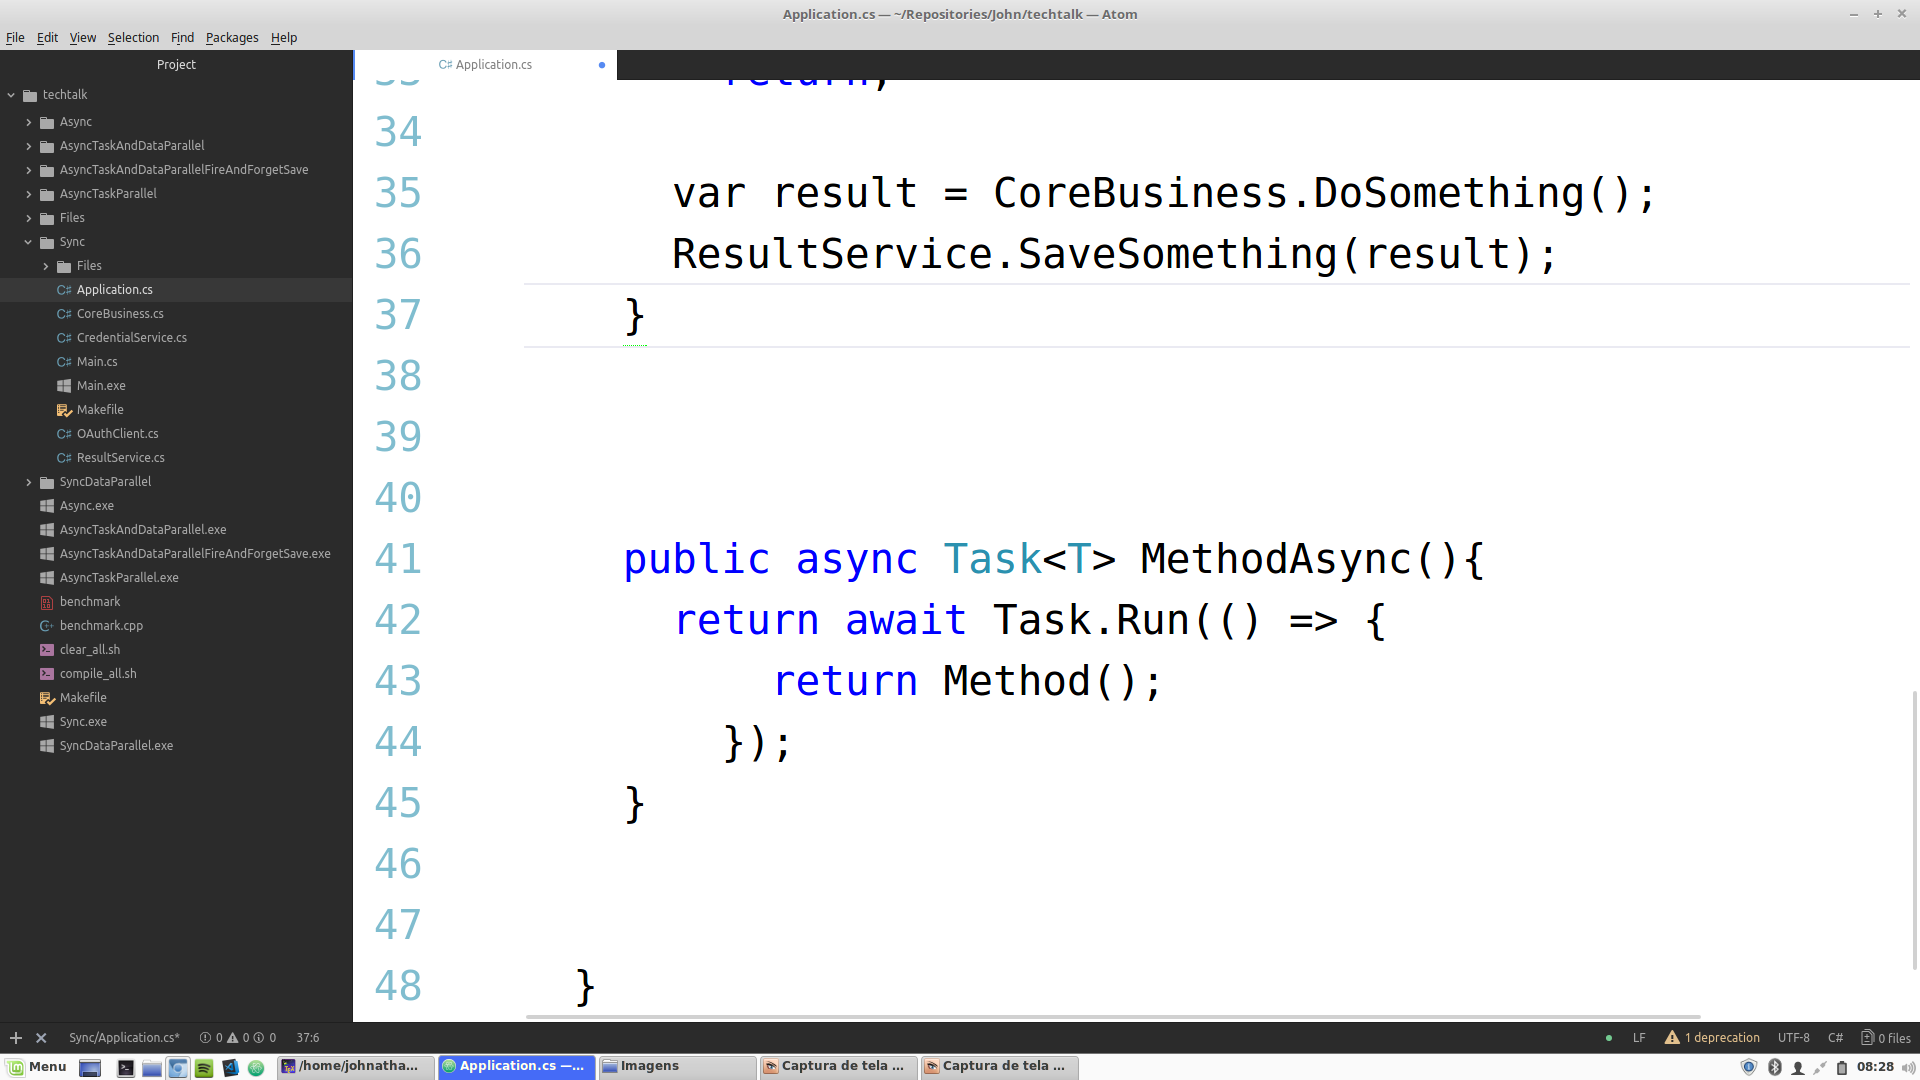
\includegraphics[width=\textwidth]{imgs/02-syncToAsync.png}
\end{frame}

\begin{frame}{Transformando código assíncrono em síncrono}
	
\includegraphics[width=\textwidth]{imgs/03-asyncToSync.png}
\end{frame}

\begin{frame}{Exemplos para Benchmark}
	\textbf{Sync x Async}
\end{frame}


\begin{frame}{Benchmark}
	\begin{figure}
		\begin{tikzpicture}
		\begin{axis}[
		mbarplot,
		ymin=0, ymax=5.4,
		%xlabel={Foo},
		ylabel={Tempo de Execução},
		width=0.9\textwidth,
		height=6cm,
		xticklabels={,,}
		]
		
		\addplot plot coordinates {(0, 5.312)};
		\addplot plot coordinates {(0, 5.361)};
		
		\legend{Sync (5.312s), Async (5.361s)}
		
		\end{axis}
		\end{tikzpicture}
	\end{figure}
\end{frame}

\begin{frame}{Fui tapeado?}
	\begin{alertblock}{Por que não houve ganhos de performance?}
		Programação Assíncrona apenas é responsável por não bloquear a execução.
	\end{alertblock}
	\vspace{0.2cm}
	\begin{exampleblock}{Então para que vou usar isso?}
		Depende da aplicação.
	\end{exampleblock}
\end{frame}

\begin{frame}{Uma requisição síncrona no WebAPI}
	
\includegraphics[width=\textwidth]{imgs/sync1}
	\begin{itemize}
		\item Uma thread livre e outra thread bloqueada realizando \textbf{nada};
	\end{itemize}
\end{frame}

\begin{frame}{Três requisições síncronas no WebAPI}
	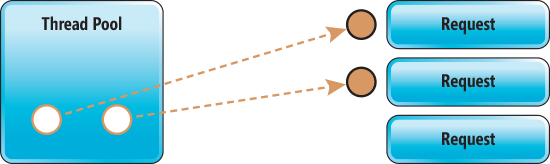
\includegraphics[width=\textwidth]{imgs/sync2}
	\begin{itemize}
		\item Duas threads bloqueadas realizando \textbf{nada} e uma requisição em espera;
	\end{itemize}
\end{frame}

\begin{frame}{Uma requisição assíncrona no WebAPI}
	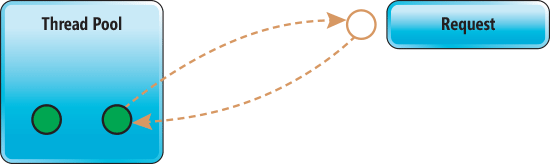
\includegraphics[width=\textwidth]{imgs/async}
	\begin{itemize}
		\item Thread realiza uma requisição bloqueante e retorna para a espera;
	\end{itemize}
\end{frame}

\begin{frame}{Ganhos}
	\begin{itemize}
		\item Redução de custos em relação à memória;
		\vspace{0.2cm}
		\item Redução do tempo de CPU desperdiçado;
	\end{itemize}
\end{frame}

\section{Paralelismo em C\#}

\begin{frame}{Paralelismo X Concorrência}
	\begin{itemize}
		\item \textbf{Paralelismo:} Duas tarefas são executadas simultaneamente.
		\begin{itemize}
			\item Executadas em diferentes processadores;
			\item Executadas em diferentes núcleos de um mesmo processador;
		\end{itemize}
		\vspace{0.2cm}
		\item \textbf{Concorrência:} Duas tarefas estão em progresso ao mesmo tempo;
		\begin{itemize}
			\item Executadas de forma alternada em um mesmo núcleo;
		\end{itemize}
	\end{itemize}
\end{frame}

\begin{frame}{Paralelismo X Concorrência}
	\begin{itemize}
		\item \textbf{Em um processador de 4 núcleos:}
		\begin{itemize}
			\item Executando 4 threads. Pode-se alocar 1 thread por núcleo;
			\vspace{0.2cm}
			\item Executadas 5 threads. Pelo menos 2 threads vão ser alternadas em um único núcleo;
		\end{itemize}
	\end{itemize}
\end{frame}

\begin{frame}{Tipos de Paralelismo}
	\begin{itemize}
		\item \textbf{Paralelismo de Dados:} A mesma instrução é executada em diferentes threads.
		\begin{itemize}
			\item Ex: Enquanto uma thread itera sobre a parte inicial de uma lista, outra itera sobre a parte final; 
		\end{itemize}
		\vspace{0.2cm}
		\item \textbf{Paralelismo de Tarefas:} Diferentes instruções são executadas em várias threads;
		\begin{itemize}
			\item Ex: Enquanto uma thread valida um token, outra busca credenciais no banco;
		\end{itemize}
	\end{itemize}
\end{frame}


\begin{frame}{Exemplo para Benchmark}
	\textbf{SyncDataParallel}
\end{frame}

\begin{frame}{Benchmark}
	\begin{figure}
		\begin{tikzpicture}
		\begin{axis}[
		mbarplot,
		ymin=0, ymax=5.5,
		%xlabel={Foo},
		ylabel={Tempo de Execução},
		width=0.9\textwidth,
		height=6cm,
		xticklabels={,,}
		]
		
		\addplot plot coordinates {(0, 5.312)};
		\addplot plot coordinates {(0, 5.361)};
		\addplot plot coordinates {(0, 3.755)};
				
		\legend{Sync (5.312s), Async (5.361s), SyncD (3.755s)}
		
		\end{axis}
		\end{tikzpicture}
	\end{figure}
	\textbf{Problemas com Async}
\end{frame}


\begin{frame}{Perguntas Frequentes}
	\begin{exampleblock}{Posso aplicar isso em qualquer problema?}
		Depende da quantidade de transformação de dados envolvida.
	\end{exampleblock}
	\vspace{0.2cm}
	\begin{exampleblock}{Quanto maior o número de threads melhor?}
		Existe um limiar onde a aplicação gasta mais tempo na comunicação entre threads do que o ganho de performance na execução paralela.
	\end{exampleblock}
\end{frame}

\section{Programação Assíncrona e Paralela em C\#}

\begin{frame}{Exemplo para Benchmark}
	\textbf{AsyncTaskAndDataParallel}
\end{frame}

\begin{frame}{Benchmark}
	\begin{figure}
		\begin{tikzpicture}
		\begin{axis}[
		mbarplot,
		ymin=0, ymax=5.5,
		%xlabel={Foo},
		ylabel={Tempo de Execução},
		width=0.9\textwidth,
		height=6cm,
		xticklabels={,,}
		]
		
		\addplot plot coordinates {(0, 5.312)};
		\addplot plot coordinates {(0, 5.361)};
		\addplot plot coordinates {(0, 3.755)};
		\addplot plot coordinates {(0, 2.579)};
		
		\legend{Sync (5.312s), Async (5.361s), SyncD (3.755s)), AsyncDT (2.579s)}
		
		\end{axis}
		\end{tikzpicture}
	\end{figure}
\end{frame}

\begin{frame}{Exemplo para Benchmark}
	\textbf{AsyncTaskAndDataParallelQueueSave}
\end{frame}

\begin{frame}{Benchmark}
	\begin{figure}
		\begin{tikzpicture}
		\begin{axis}[
		mbarplot,
		ymin=0, ymax=5.5,
		%xlabel={Foo},
		ylabel={Tempo de Execução},
		width=0.9\textwidth,
		height=6cm,
		xticklabels={,,}
		]
		
		\addplot plot coordinates {(0, 5.312)};
		\addplot plot coordinates {(0, 5.361)};
		\addplot plot coordinates {(0, 3.755)};
		\addplot plot coordinates {(0, 2.579)};
		\addplot plot coordinates {(0, 1.588)};
			
		\legend{Sync (5.312s), Async (5.361s), SyncD (3.755s), AsyncDT (2.579s), AsyncDTQS (1.588s)}
		
		\end{axis}
		\end{tikzpicture}
	\end{figure}
	\textbf{QueueWork != Async sem Await}
\end{frame}

\section{Conclusões}

\begin{frame}{Conclusões}
	\begin{itemize}
		\item É possível criar métodos assíncronos e paralelos no WebAPI de forma simples e conveniente; 
		\item Métodos assíncronos devem ser utilizados em APIs com finalidade de otimizar a utilização de recursos;
		\item Paralelismo nunca fornece um ganho linear de performance e deve ser utilizado em problemas onde a quantidade de transformações de dados é grande;
	\end{itemize}
\end{frame}


\begin{frame}[standout]
  Perguntas?
\end{frame}

\end{document}
